\documentclass[11pt]{article}
\usepackage{mytex}
\usepackage{fullpage}
\usepackage{graphicx}
\usepackage{enumitem}
\usepackage{color,soul}

\begin{document}
%\newcommand{\answer}[1]{{\bf (Answer: #1)}}
\newcommand{\answer}[1]{\mbox{~}}

{\large  CSCE 464 Wireless and Mobile Systems  \hfill Fall 2020\\
 \begin{center}
   Homework 1 \\
   Bryan Lara \\
    \end{center}
}

\section{Signal Encoding}
\begin{enumerate}[label=(\alph*)]
\item 
\begin{itemize}
  \item 2.3- Why does the ITU-R only regulate ‘lower’ frequencies (up to some hundred GHz)
and not higher frequencies (in the THz range)?
    \begin{itemize}
         \item  This is because at the THz  range we get to frequencies that can not pass through object as easily and as strong as lower frequencies. Therefore, it is less likely to cause interference, thus not much regulation is needed.
    \end{itemize}
  \item 2.8- What are the main problems of signal propagation? Why do radio waves not
always follow a straight line? Why is reflection both useful and harmful?
    \begin{itemize}
        \item Frequently causing transmission errors and propagation not predictable unless in vacuum.
        Radio waves deal with "Sky wave" propagation. Radio waves reflect of the ionosphere and bounce between it and the earth's surface. Reflection can be harmful in cases where a signal was suppose to travel through the point it was reflected from, causing the transmission field to decrease. Reflection can be also be used to get signal around an object that would otherwise make it impossible for the the signal to get to. Also in the case of radio waves, the signal can continue reflecting between the ionosphere and ground to reach further distances.
    \end{itemize}
  \item 2.9-  Name several methods for ISI mitigation. How does ISI depend on the carrier frequency, symbol rate, and movement of sender/receiver? What are the influences
of ISI on TDM schemes?
    \begin{itemize}
        \item For ISI mitigation we can use,multi-carrier modulation (MCM), COFDM, guard spaces, higher frequencies,and a training sequence. Higher symbol rate causes worse effects of ISI. If receiver or transmitter is moving, ISI worsen. With higher carrier frequency, ISI affects can be lessened like in MCM.For TDM, we have to make sure that our gaurd spaces in time are enough to not be affected by ISI.
        
        
    \end{itemize}
  \item 2.12- Think of a phase diagram and the points representing bit patterns for a PSK
scheme (see Figure 2.29). How can a receiver decide which bit pattern was originally sent when a received ‘point’ lies somewhere in between other points in the
diagram? Why is it difficult to code more and more bits per phase shift?
    \begin{itemize}
        \item The receiver can utilize maximum likely hood detection to determine what bit pattern was originally sent.It becomes more difficult to separate the points as you add more points in the quadrants.
    \end{itemize}
\end{itemize}

\item  
\begin{itemize}
    \item {\(1.25*10^{-4}W = 1.25*10^{-1}mW = 10*log_{10}(1.25*10^{-1}) dBm = -9.031 dBm\)}
    \item {\(2.5*10^{-4}W = -6.0206 dBm\)}
    \item {\(5*10^{-4}W = -3.0103 dBm\)}
    \item {\(1*10^{-3}W = 0 dBm\)}
    \item {\(2*10^{-3}W = 3.0103 dBm\)}
    \item {\(4*10^{-3}W = 6.0206 dBm\)}
    \item {\(8*10^{-3}W = 9.031 dBm\)}
    \item The pattern I see is that the value to the left and right of 1mW is inverted.
    
\end{itemize}
\item .\\
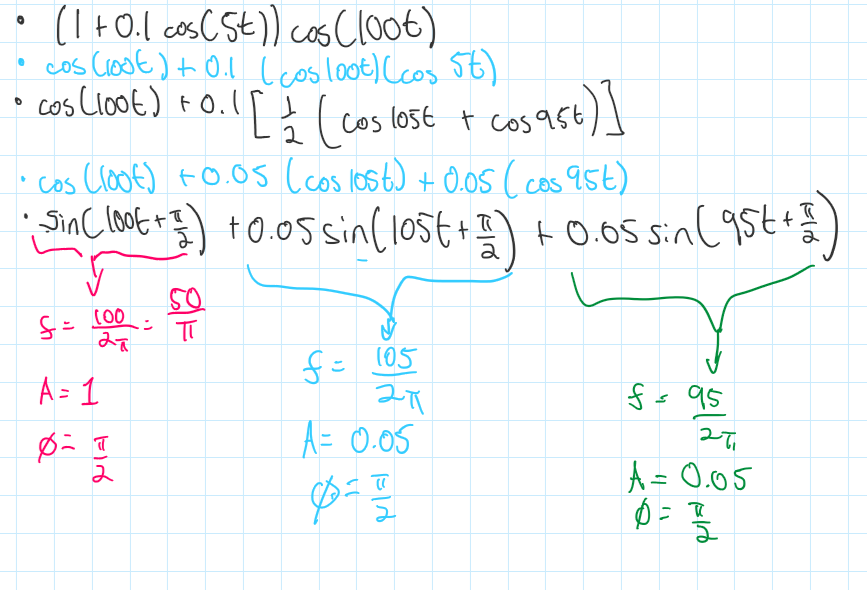
\includegraphics[width=0.9\textwidth]{1c}
 
\item For binary value representation in ASK, a binary 0 would be represented with a small to no amplitude while a binary 1 would be represented with a sinusoidal signal with a large amplitude.This method is an inefficient modulation technique and is susceptible to sudden gain changes. It is also significantly affected by noise.
\\ \\ \\ \\ \\ \\ \\ \\ \\ \\ \\ \break

\item . \\
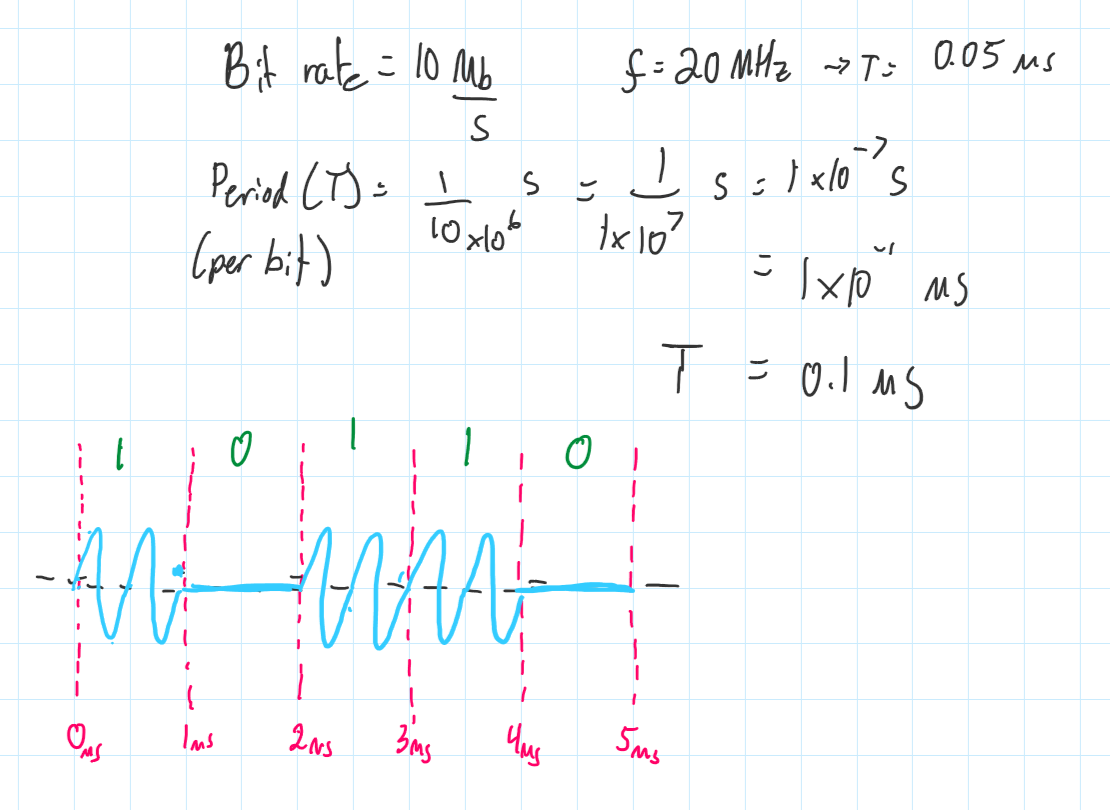
\includegraphics[width=0.9\textwidth]{1e}
\item . \\
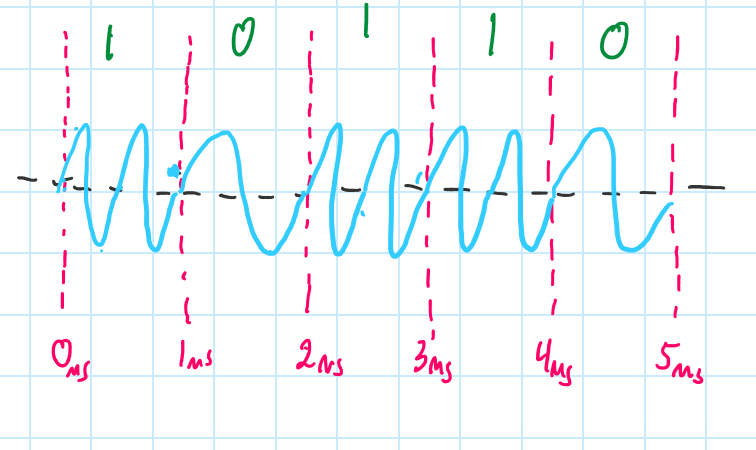
\includegraphics[width=0.9\textwidth]{1f} \\
\item .\\
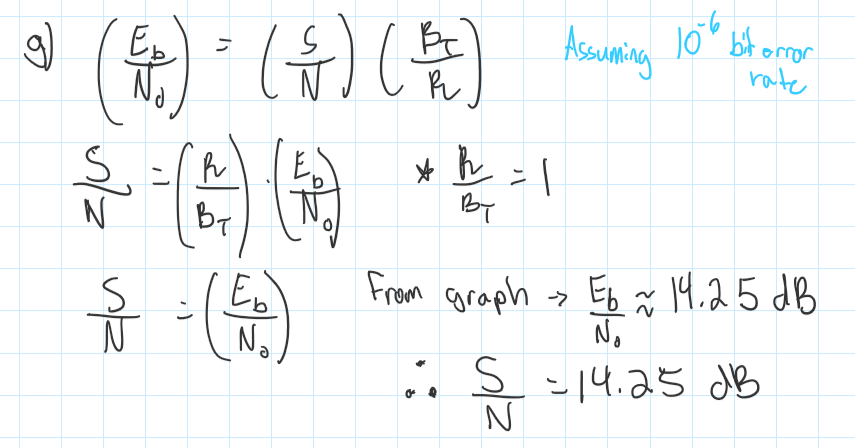
\includegraphics[width=0.9\textwidth]{1g} \\

\begin{center}
    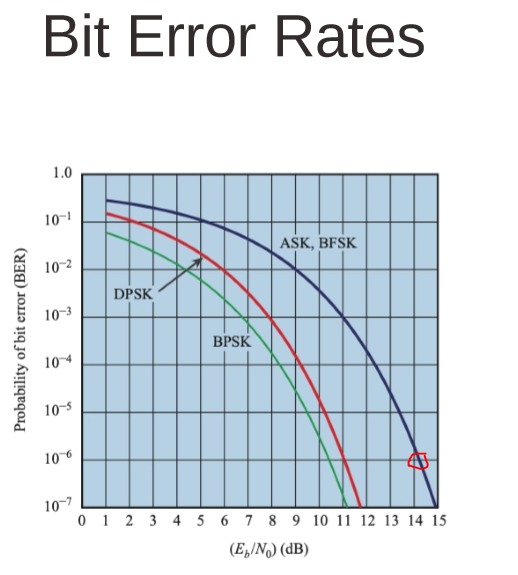
\includegraphics[width=0.5\textwidth]{1ga}
\end{center}

\end{enumerate}
 


\section{Channel Capacity, Models}
\begin{enumerate}[label=(\alph*)]
\item .\\
    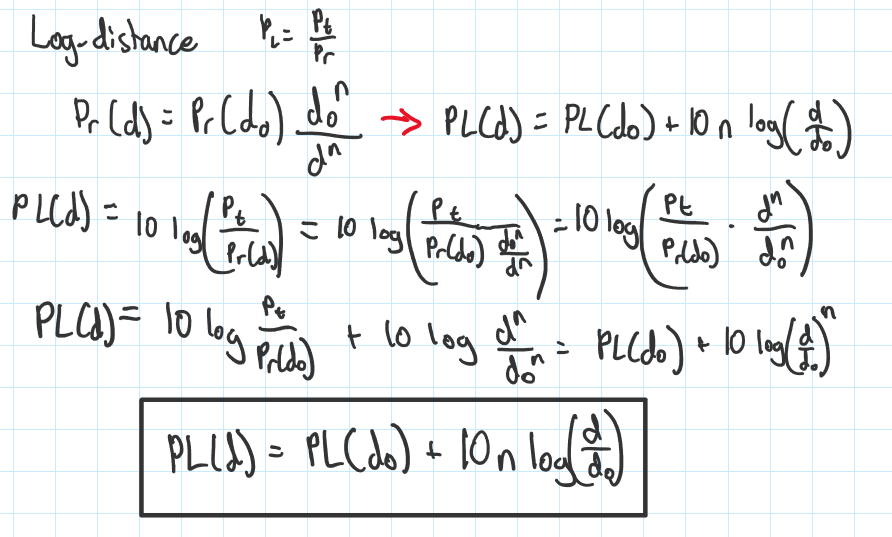
\includegraphics[width=0.9\textwidth]{2a}\\
\item  .\\
    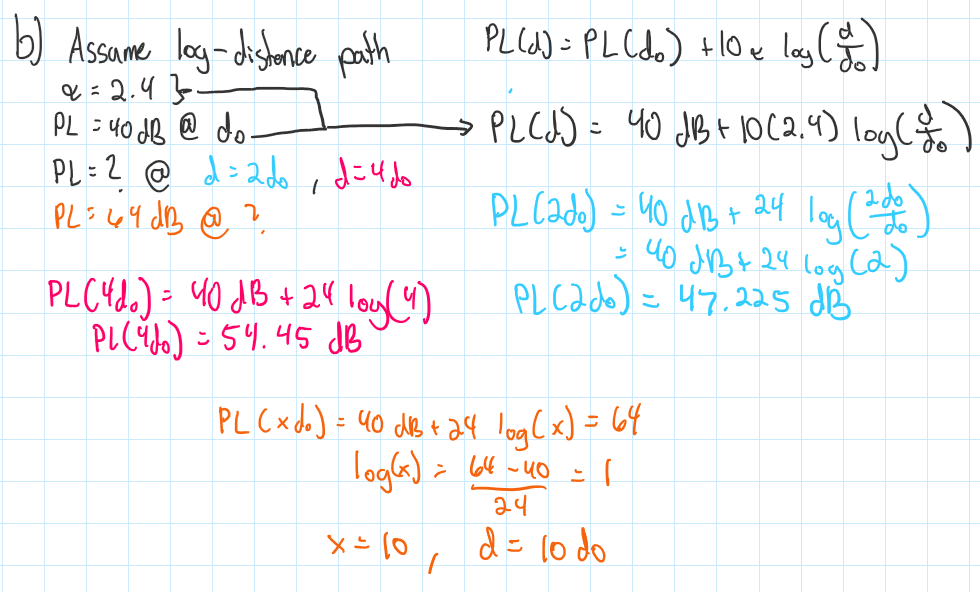
\includegraphics[width=0.9\textwidth]{2b}\\
\item  .\\
    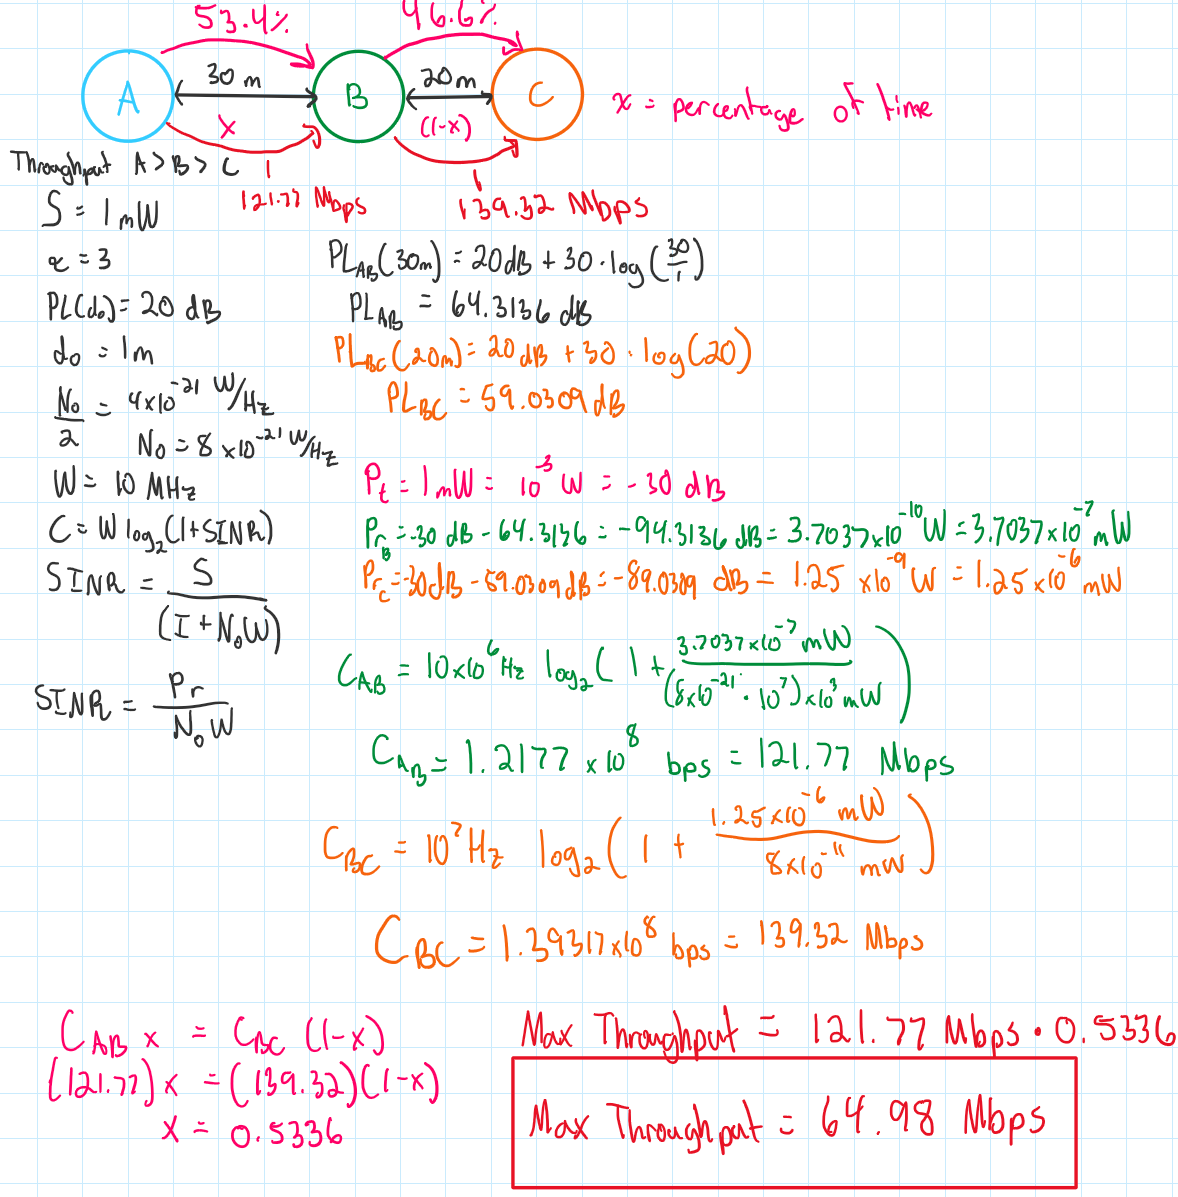
\includegraphics[width=1\textwidth]{2c}\\\\\\\\\\\\\\\\
\item .\\ 
    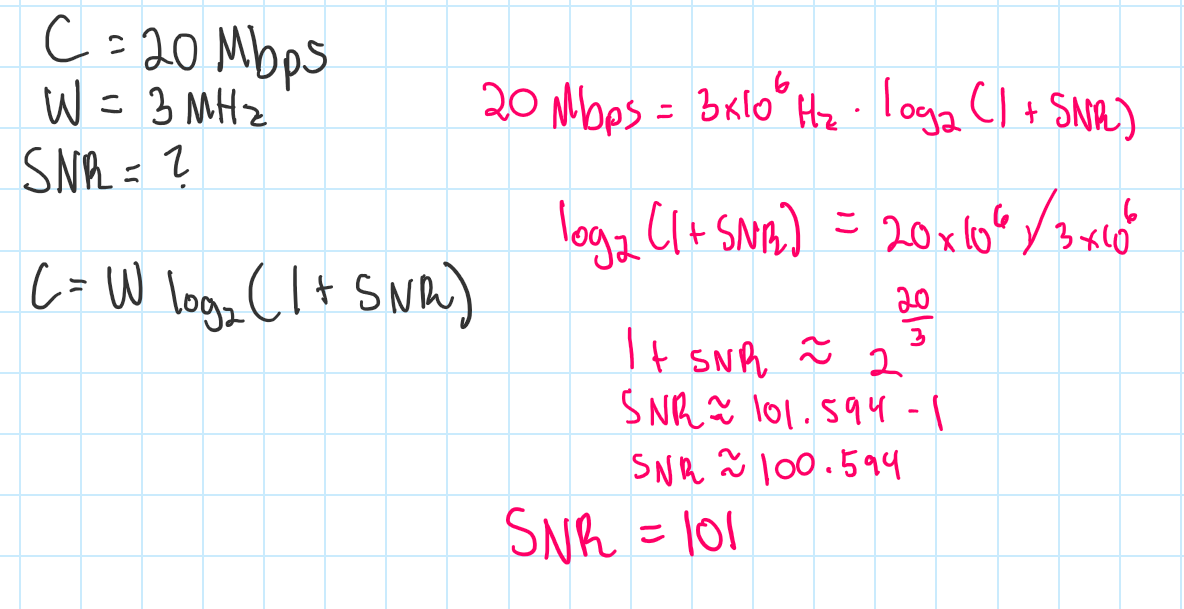
\includegraphics[width=1\textwidth]{2d}\\
\end{enumerate}
	

\section{Coding and Error Control}
\begin{center}
    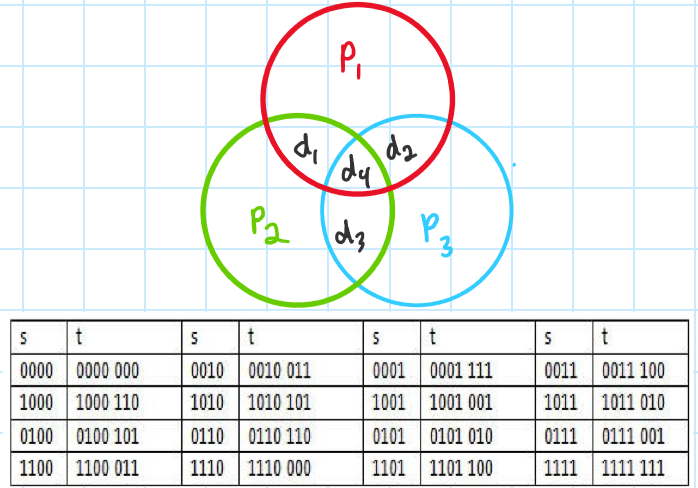
\includegraphics[width=1\textwidth]{3x}
\end{center}
\begin{enumerate}[label=(\alph*)]
\item .\\ 
    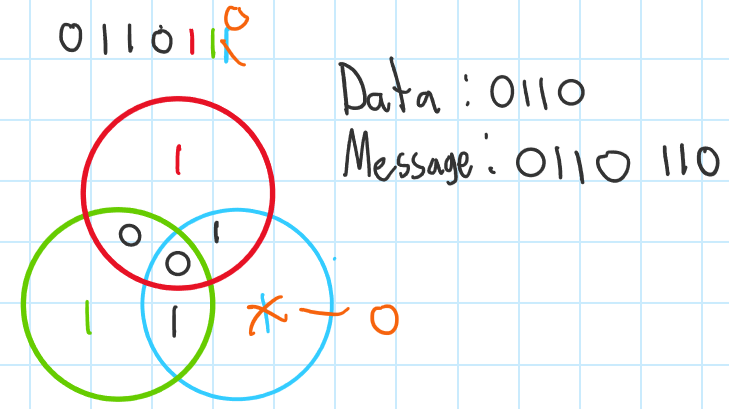
\includegraphics[width=.9\textwidth]{3a}
\item .\\ 
    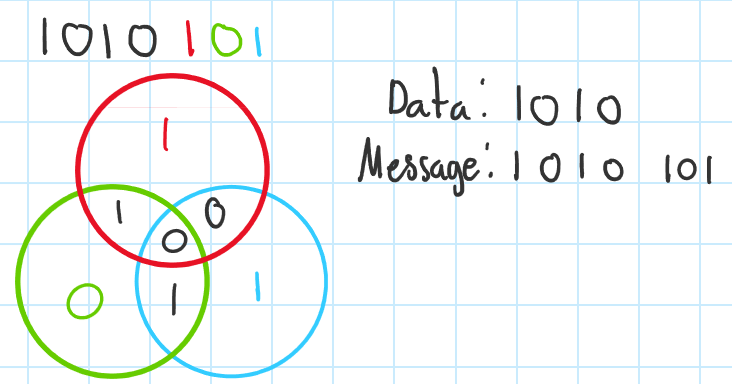
\includegraphics[width=.5\textwidth]{3b}
\item .\\ 
    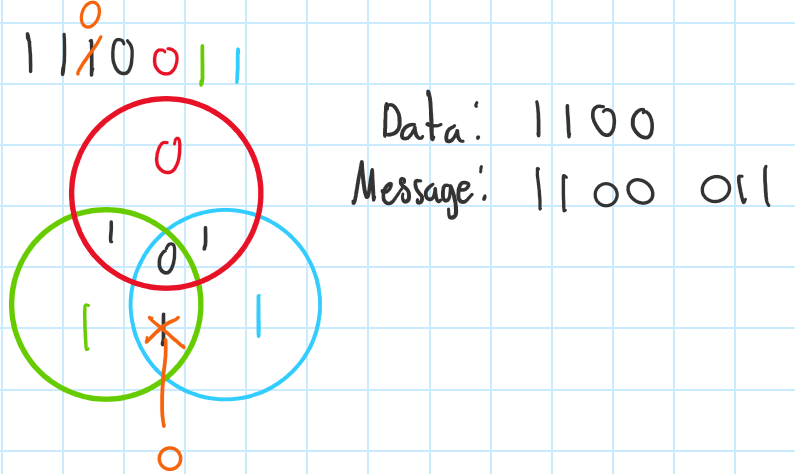
\includegraphics[width=.5\textwidth]{3c}
\item .\\ 
    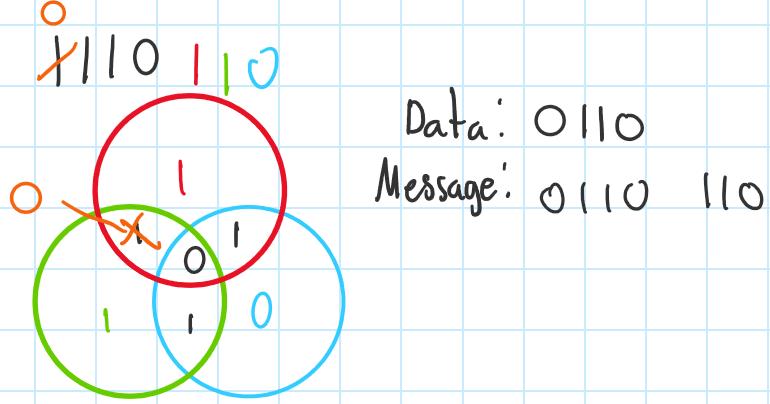
\includegraphics[width=.5\textwidth]{3d}
\item .\\ 
    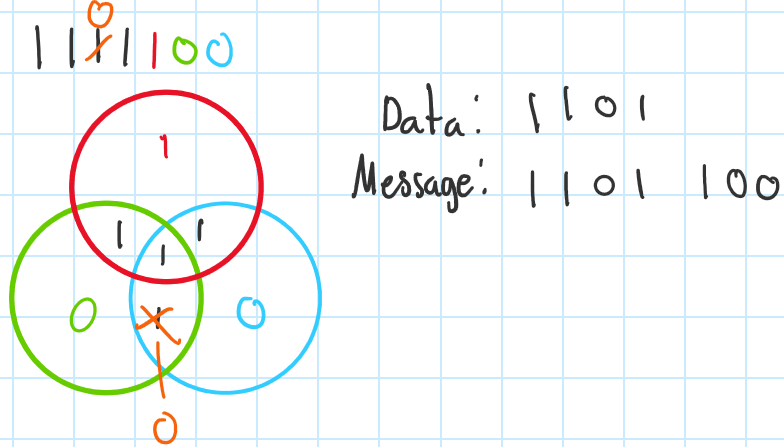
\includegraphics[width=.5\textwidth]{3e}
\end{enumerate}

\section{Wireshark}
\begin{enumerate}[label=(\alph*)]
\item Intro 
\begin{center}
    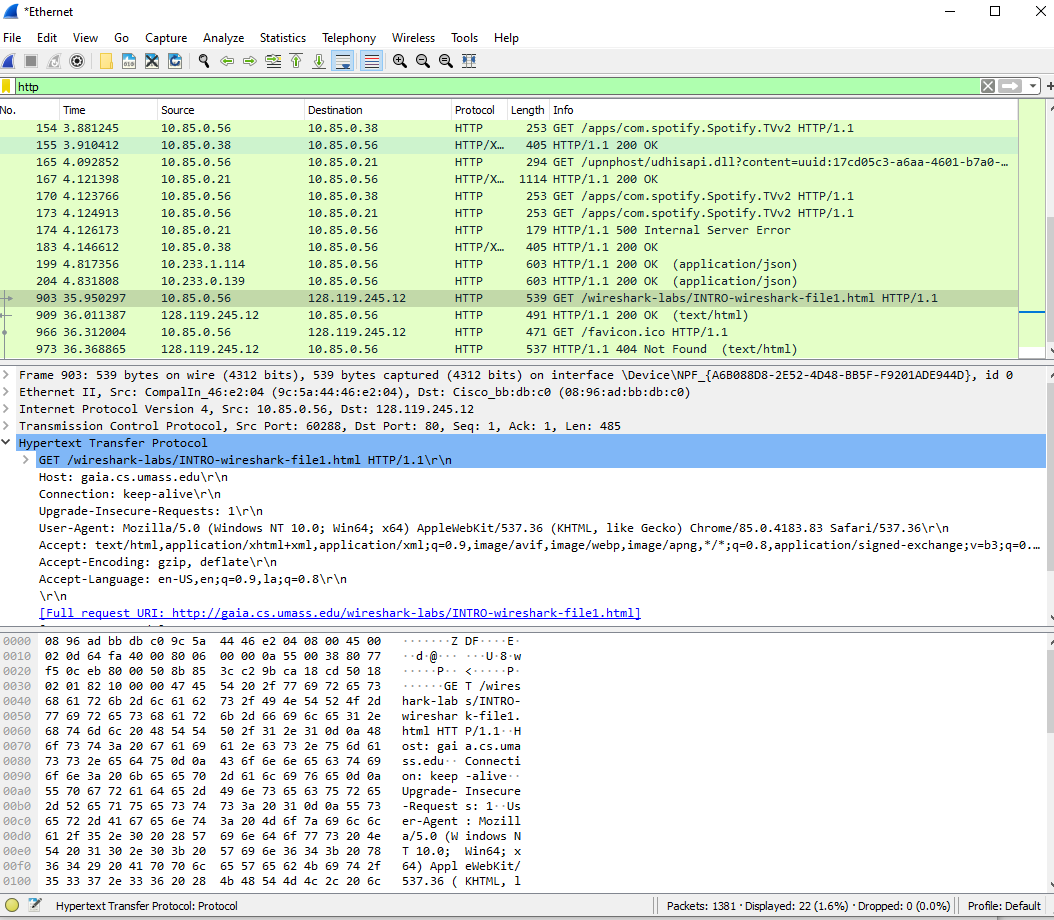
\includegraphics[width=.9\textwidth]{HW1Template/Wireshark_Intro.PNG}
\end{center}
\begin{enumerate}[label=(\arabic*)]
    \item List 3 different protocols that appear in the protocol column in the unfiltered
packet-listing window in step 7 above.
        \begin{itemize}
            \item TCP, UDP, STP, TLSv1.2/v1.3, MDNS, HTTP, NBNS, LLMNR. DNS, SSDP, ARP, AJP13
        \end{itemize}
    \item How long did it take from when the HTTP GET message was sent until the HTTP
OK reply was received?
    \begin{itemize}
        \item It took 0.06109s or 61.1ms.
    \end{itemize}
    
    \item What is the Internet address of the gaia.cs.umass.edu (also known as wwwnet.
cs.umass.edu)? What is the Internet address of your computer?
    \begin{itemize}
        \item gaia.cs.umass.edu address: 128.119.245.12
        \item My computer address : 10.85.0.56
    \end{itemize}
    
    \item Print the two HTTP messages (GET and OK) referred to in question 2 above. To
do so, select Print from the Wireshark File command menu, and select the
“Selected Packet Only” and “Print as displayed” radial buttons, and then click
OK.\\
 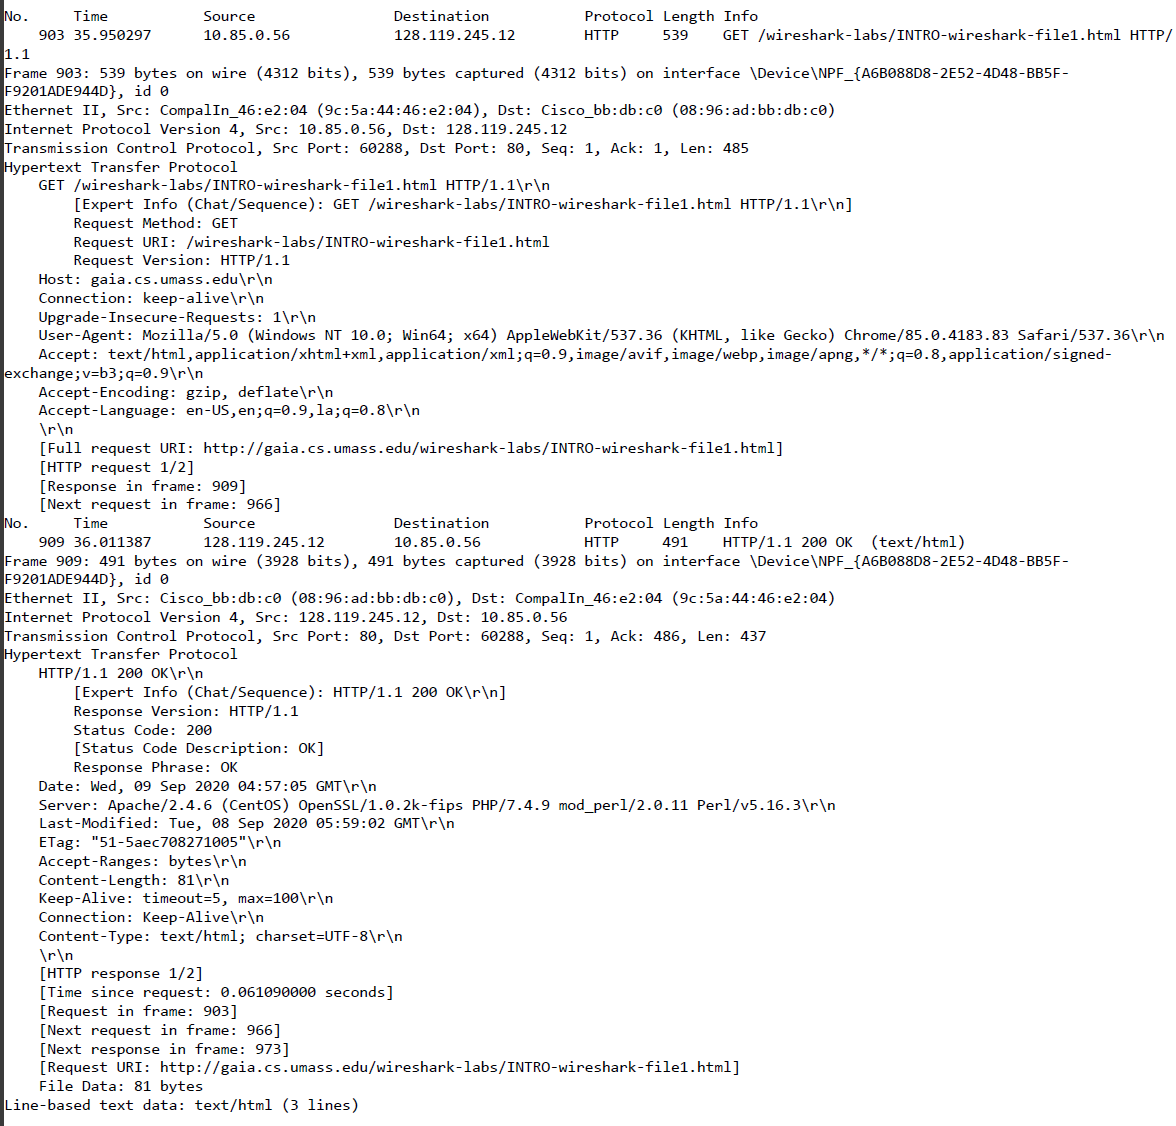
\includegraphics[width=1\textwidth]{HW1Template/Wireshark_Intro_4.PNG}
   
    
    
    
\end{enumerate}
    \newpage
\item WireShark ICMP
    \begin{itemize}
        \item Section ICMP and Ping\\
        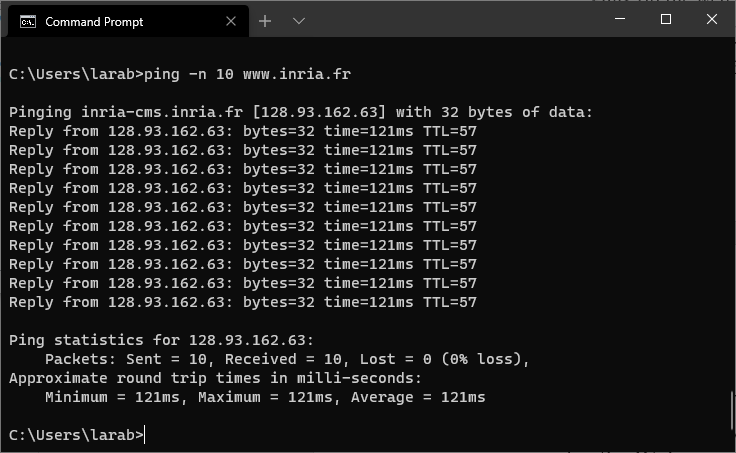
\includegraphics[width=1\textwidth]{HW1Template/wireshark_ping.PNG}
        
        \begin{enumerate}[label=(\arabic*)]
            \item What is the IP address of your host? What is the IP address of the destination host? 
                \begin{itemize}
                    \item My IP Address: 10.85.0.56
                    \item Host IP Address: 128.93.162.63
                \end{itemize}
            \item Why is it that an ICMP packet does not have source and destination port numbers? 
                \begin{itemize}
                    \item This is because the ICMP protocal was design for the communicate network-layer between host and router, not the application layer
                \end{itemize}
                \begin{center}
                    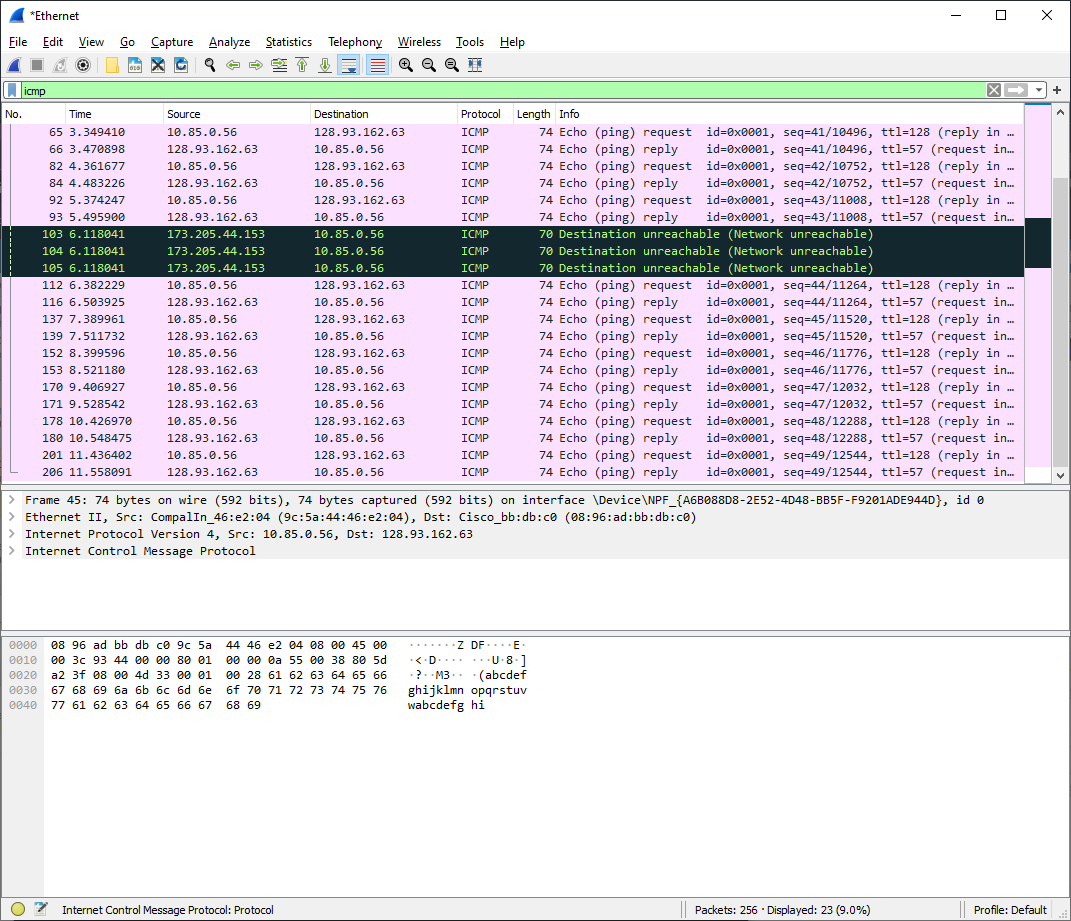
\includegraphics[width=1\textwidth]{HW1Template/wireshark_ping_capture.PNG}
                \end{center}
                
            \item Examine one of the ping request packets sent by your host. What are the ICMP type and code numbers? What other fields does this ICMP packet have? How many bytes are the checksum, sequence number and identifier fields?
                \begin{itemize}
                    \item ICMP type: 8 (Echo (pipng) request)
                    \item ICMP code: 0
                    \item Has Checksum, Identifier, Sequence number, and data(32 bytes)
                    \item Checksum: 4bytes, Sequence(BE/LE): 4bytes, Identifier(BE/LE): 4bytes
                \end{itemize}
            \item Examine the corresponding ping reply packet. What are the ICMP type and code numbers? What other fields does this ICMP packet have? How many bytes are the checksum, sequence number and identifier fields?
                \begin{itemize}
                    \item Type: 0 (Echo (ping) reply)
                    \item Code: 9
                    \item Has Checksum, Identifier, Sequence number, and data(32 bytes)
                    \item Checksum: 4bytes, Sequence(BE/LE): 4bytes, Identifier(BE/LE): 4bytes
                \end{itemize}
            
        \end{enumerate}
         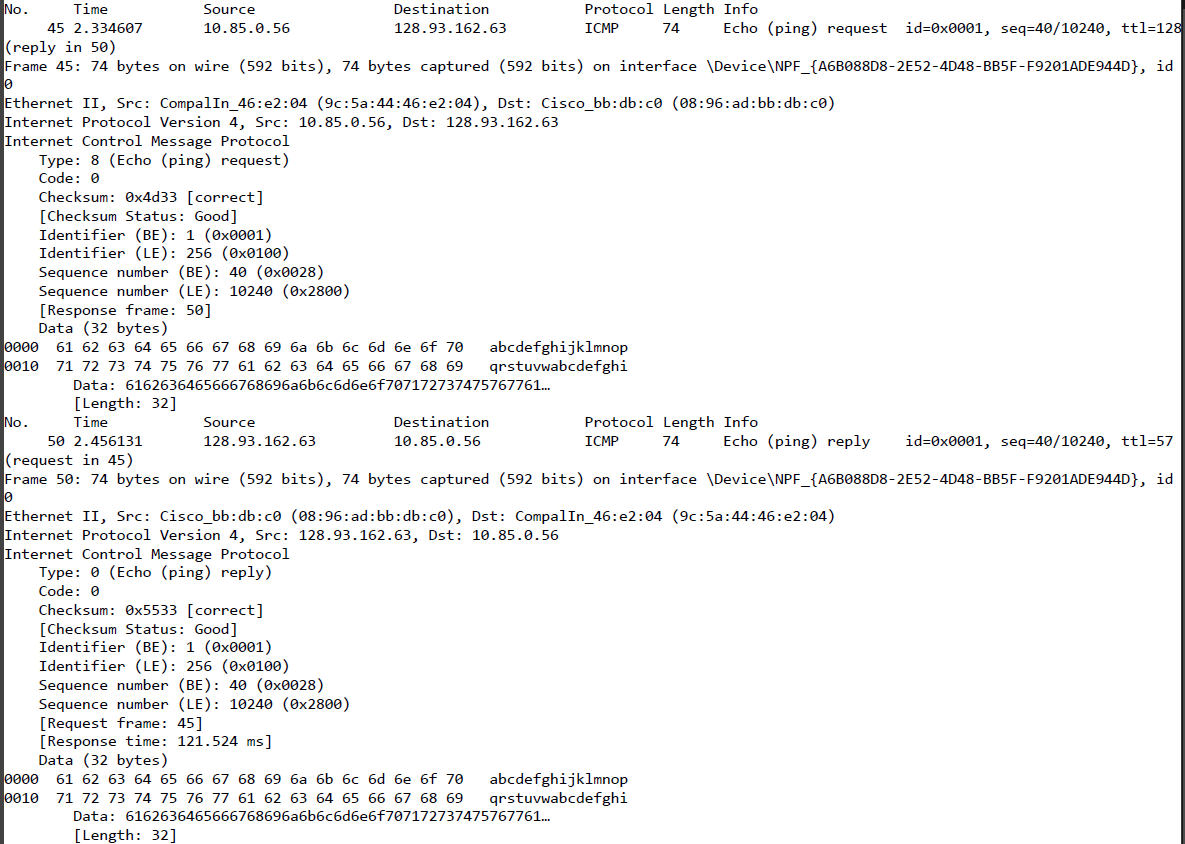
\includegraphics[width=1\textwidth]{HW1Template/Wireshark_ping_print.PNG}
        
        
        \item Section ICMP and Traceroute \\ \\
        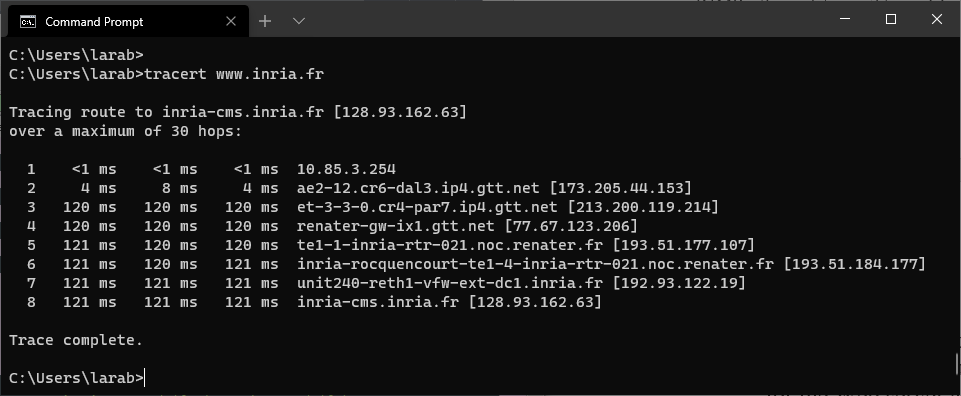
\includegraphics[width=1\textwidth]{HW1Template/trace_cmd.PNG}
        \begin{enumerate}[label=(\arabic*)]
        \setcounter{enumii}{4}
            \item What is the IP address of your host? What is the IP address of the target destination host?
                \begin{itemize}
                    \item My IP Address: 10.85.0.56
                    \item Host IP Address: 128.93.162.63
                \end{itemize}
                
                
            \item If ICMP sent UDP packets instead (as in Unix/Linux), would the IP protocol number still be 01 for the probe packets? If not, what would it be? 
                \begin{itemize}
                    \item If UDP packets were sent, the IP protocol number would change from (1) to (17)
                \end{itemize}
                
                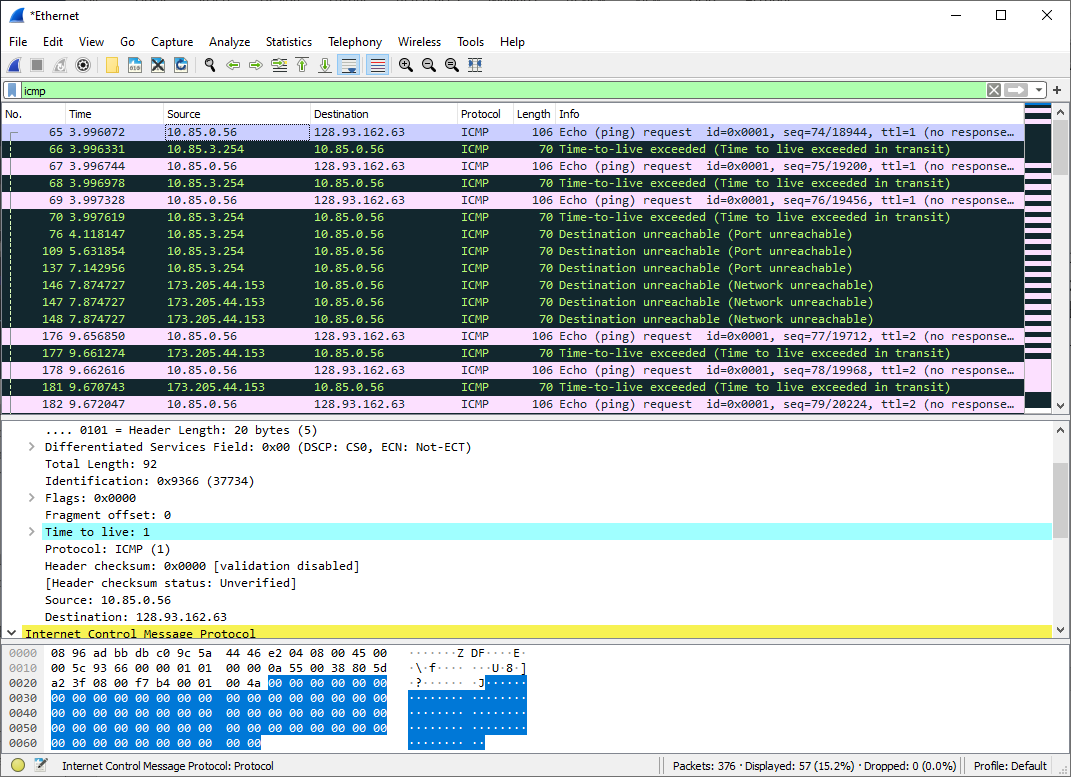
\includegraphics[width=1\textwidth]{HW1Template/wireshark_trace_capture.PNG}
            \item Examine the ICMP echo packet in your screenshot. Is this different from the ICMP ping query packets in the first half of this lab? If yes, how so?
                \begin{itemize}
                    \item The ICMP echo packet looks the same as the ICMP ping query from earlier.
                \end{itemize}
                
                
            \item Examine the ICMP error packet in your screenshot. It has more fields than the ICMP echo packet. What is included in those fields?
                \begin{itemize}
                    \item The extra fields it has are the IP header and the ICMP packet that was the time out error was caused by.
                \end{itemize}
                
                
            \item Examine the last three ICMP packets received by the source host. How are these packets different from the ICMP error packets? Why are they different?
                \begin{itemize}
                    \item These packets are Type: 0 (Echo (ping) reply) and contain data(64 bytes) because the packets were successfully able to be routed and not time out.
                \end{itemize}
                
                
            \item Within the tracert measurements, is there a link whose delay is significantly longer than others?  Refer to the screenshot in Figure 4, is there a link whose delay is significantly longer than others?  On the basis of the router names, can you guess the location of the two routers on the end of this link?
                \begin{itemize}
                    \item There is a significant delay between step 2 and 3. Using en.ipip.net step 2 is from Dallas to step 3 in Paris which explains the delay.
                \end{itemize}
            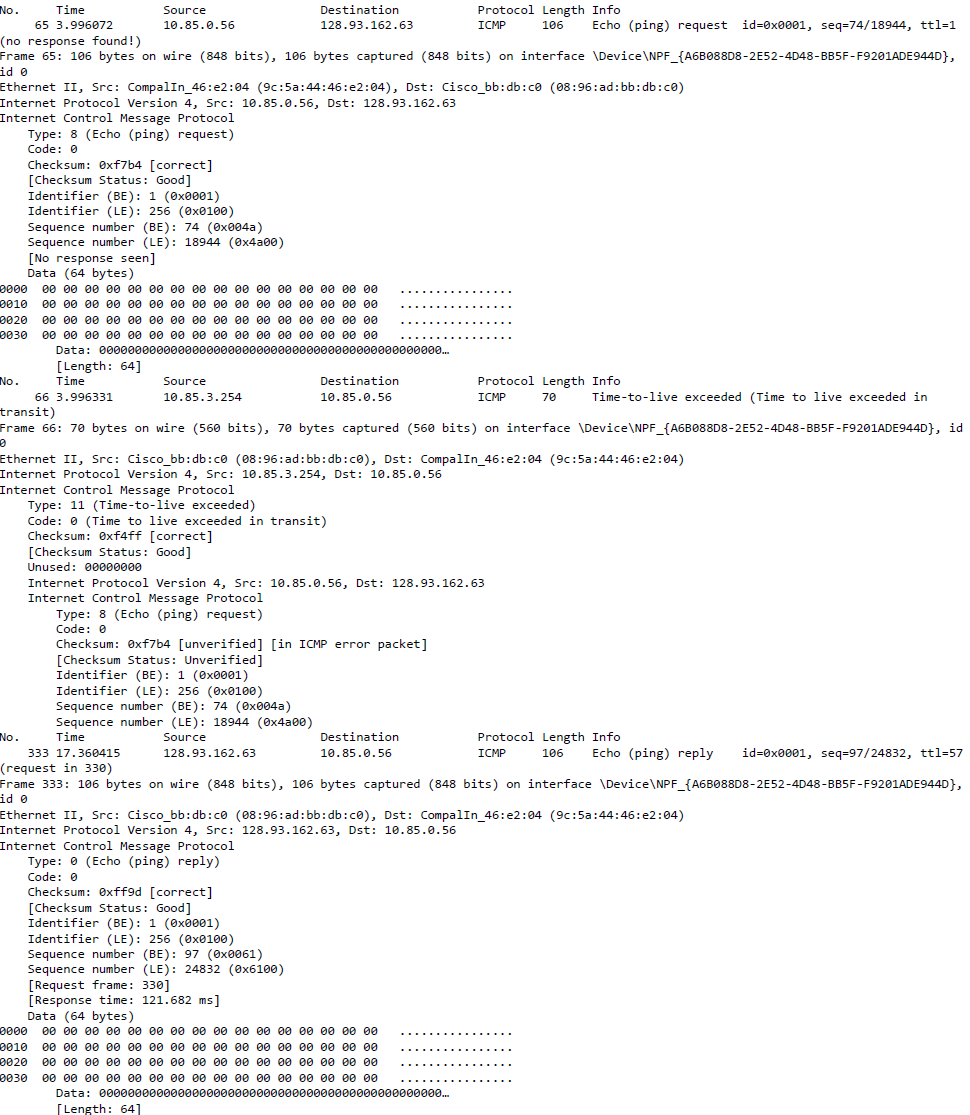
\includegraphics[width=1\textwidth]{HW1Template/Wireshark_trace_print.PNG}
            
        \end{enumerate}
    \end{itemize}
\end{enumerate}


\end{document}

